\documentclass{ctexart}
\usepackage{amsmath,amsfonts,amssymb,bm,indentfirst,hyperref}
\usepackage[cache=false]{minted}
\usepackage{algorithm,algorithmic}
\usepackage{graphicx}
\title{计算物理大作业}
\author{王宇逸\ 谷海桥\ 李禹苏}
\bibliographystyle{plain}
\begin{document}
\maketitle
\newpage
\tableofcontents
\newpage

\begin{abstract}
    我们研究了由D.W.Brenner等人开发的分子动力学框架BrennerMD,分析了程序结构、使用算法,并使用程序进行了一定的模拟。
    通过这一过程,更好地理解了分子动力学方法及其应用。
\end{abstract}

\section{框架概述}
BrennerMD是由D.W.Brenner等人使用FORTRAN 77开发的分子动力学开源框架。
尽管框架开源,但是由于年代久远,在互联网上难觅踪迹。
现在唯一能找到源代码的网站在SourceForge.Net上(\url{https://sourceforge.net/projects/brennermd/})。
这个网站给出了源代码,并使用C语言重写了一份。

FORTRAN 77是年代久远的数学编程语言。在那个还使用着打孔纸带的年代,有这样一门对数学运算友好的高级语言,一定是开发人员的首选。
然而时过境迁,在现代人的眼光看来,FORTRAN 77对机器的软硬件所做的语法层面的妥协极不合理,而Fortran也在一次次版本迭代中与曾经的标准面目全非。
因此,使用FORTRAN 77的框架鲜有人问津,只有一些“祖传”的代码因为难读、难改、组织混乱,而一直流传至今。

\section{程序流程与结构}
程序代码文件分为两部分。
Execute文件夹提供了一份能够编译通过的代码,但是这些代码文件平铺在同一个文件夹中,比较混乱;
Subroutines等文件夹又将这些代码文件按照功能分类,并给出了基本的README文件作为介绍。
在Execute文件夹内,运行
\begin{minted}{bash}
    $ gfortran main.f -o main.x -std=legacy -g
\end{minted}
生成main.x可执行程序。
“-g”选项加入调试符号,是为了在程序崩溃(这种情况经常发生)的时候给出清楚的调用栈。

main.f文件内是程序的主函数,大致分为初始化与计算两部分,下面就这两部分分别介绍
\subsection{初始化}
初始化的步骤比较简单,按照如下顺序依次执行:
\begin{minted}{fortran}
    include 'open.inc'
\end{minted}
打开所有文件,并使用写死的、无规律的数字为其编号。
\begin{minted}{fortran}
    call setin
\end{minted}
setin函数初始化一些矩阵与常数。常数包括常用的粒子质量、$\pi$、玻尔兹曼常数等等。
\begin{minted}{fortran}
    call read_data
\end{minted}
read\_data函数读入两个文件的内容:编号为13的input.d与编号为11的coord.d。
input.d记录了一些基本的模拟参数,如步数、记录步长间隔、初始温度、使用算法、使用框架等等,以及可选地更改一些粒子的基本属性。
coord.d的输入输出在同一个文件,用于连续运行程序来模拟。包括文件头、粒子个数、时长、每一步的时间间隔、环境大小、初始坐标、速度、加速度、急动度等。
读入工作有可能有参数不合理的地方,这个时候会直接报错并退出,使用类似
\begin{minted}{fortran}
    include 'close.inc'
    stop
\end{minted}
的模式进行清理并退出。
\begin{minted}{fortran}
    call setpp
    call setpc
    call setgle
\end{minted}
setpp设置势函数的参数,主要是LJ势。
setpc设置预测器校正参数。
setgle设置朗之万参数。
\begin{minted}{fortran}
    call setran
\end{minted}
setran初始化随机数。
首先使用读入的随机数中子pseed,调用setrn进行初始化;之后的随机数调用rannum即可。
pseed也使用rannum更新一次,以保证下一次的种子与这次不同

需要指出,rannum函数虽然接受一个参数,但是它并没有使用。
更有趣的一点是,当我们搜索这个算法的时候,只能找到相同的代码,甚至注释都一样。
那些函数无一例外都有这个没有被使用的参数。

\subsection{计算}
计算过程分两种情况,根据KFLAG标志分别运行不同的算法,KFALG的具体含义可参见THERMOS部分。

\begin{enumerate}
    \item KFLAG为6时调用minimize算法

    \item 否则调用预测—校正算法进行分子动力学模拟:
\end{enumerate}



\begin{minted}{fortran}
    call setmd
\end{minted}
调用setmd,初始化相关的参数设置并打印输出信息的表头。
\begin{minted}{fortran}
    DO LSTEP=1,KVC
        call cpred  
        CALL MODEL 
        call thermos 
        call ccorr
        if(mod(LSTEP,nxmol).eq.0) call xmol
        IF(KFLAG.EQ.5) CALL BERE
        if(mod(LSTEP,maxkb).eq.0) then
            call write_data2 
        endif  
!          call vscale 
        ENDDO
\end{minted}
随后进行KVC次循环模拟运动轨迹,采用预测校正算法。每次循环的主要流程为如下:

首先调用cpred进行位置、速度、加速度的预测,MODEL根据预测的位置信息计算每个原子x,y,z方向的受力,随后调用thermos引入热力学演化,最后调用ccorr对预测的位置、速度、加速度信息进行修正。

每隔nxmol步调用xmol在xmol.d中打印坐标信息记录中间过程(若出现异常可以观察中间结果),每隔maxkb步打印步长、平均能量、动能、时间等相关信息。

\begin{minted}{fortran}
    call write_data3
\end{minted}
最后调用write\_data3打印模拟结束后的最终坐标、速度、加速度、急动度等信息覆盖coord.d。

\section{程序算法}
\subsection{能量最小化}

算法的流程

初始化,赋初值

计算初始能量与受力

求解稳定构形及最小能量

调整坐标

其中求解稳定构形及最小能量是这个子例程的核心,他主要应用了BFGS

\subsubsection{算法原理}

该程序使用的法为\textbf{BFGS},具体原理如下:

本质上是牛顿法的变形
因为能量最小的点能量的导数是0,所以问题转化成一个求根问题,

具体数学形式


\begin{eqnarray}
    H_{k}^{DFGS} &=& H_{k-1}^{DFGS} + \frac{1}{s_{k-1}^{T}y_{k-1}}[1+\frac{y_{k-1}^{T}H_{k-1}^{DFGS}y_{k-1}}{s_{k-1}^{T}y_{k-1}}]s_{k-1}s_{k-1}^{T}\nonumber\\
    &&-\frac{1}{s_{k-1}^{T}y_{k-1}}(s_{k-1}y_{k-1}^{T}H_{k-1}^{DFGS}+H_{k-1}^{DFGS}y_{k-1}s_{k-1}^{T})d_{k}^{DFGS}\nonumber\\
    &=& -H_{k}^{DFGS}g_{k}
\end{eqnarray}

简化的程序实现

\begin{algorithm}
    \begin{algorithmic}
        \STATE $x[0] \leftarrow guess$
        \STATE $b[0] \leftarrow I$
        \FOR{k}
        \STATE $s[k] \leftarrow b[k]^{-1} \nabla f(x[k])$
        \STATE $x[k+1] \leftarrow x[k] + s[k]$
        \STATE $y[k] \leftarrow \nabla f(x[k+1]) - \nabla f(x[k])$
        \STATE $b[k+1] \leftarrow b[k] + \frac{y[k]y[k]^{T}}{y[k]^{T}s[k]} - \frac{b[k]s[k]s[k]^{T}b[k]}{s[k]^{T}b[k]s[k]}$
        \ENDFOR
    \end{algorithmic}
\end{algorithm}

\subsubsection{程序实现}
\noindent
\textbf{CONMIN}

\noindent
相关参数
\begin{itemize}
    \item N:THE NUMBER OF VARIABLES IN THE FUNCTION TO BE MINIMIZED.
    \item X:双精度 N维矢量,保存当前得到的最小值的估计值的坐标位置;
    \item F:双精度。当完成 CONMIN 时,F 将保存得到的目标函数的最小值
    \item G:双精度 N维矢量。当完成 CONMIN 时,G 保存此时 X 点的梯度
    \item IFUN:保存跳出 CONMIN 时总共做过的步数
    \item IOUT: 用户设置的输出参数。
    \item RNP(I,J):第 I 个原子在第 J 维上受到的力
    \item NFLAG:跳出 CONMIN 的具体原因。
          \begin{itemize}
              \item NFLAG=0:算法已收敛。
              \item NFLAG=1:已经完成了预置的最大迭代数。
              \item NFLAG=2:线性搜索失败。函数或梯度没有被正确地编程计算通常会导致此情况。
              \item NFLAG=3:搜索方向不是最速下降方向。只可能由舍入误差引起,说明收敛精度 设置过高。
          \end{itemize}
\end{itemize}

\subsection{预测—校正算法}

算法的流程上文已经提到,这里主要关注该算法的原理以及具体实现

\subsubsection{算法原理}

该程序使用的预测—校正算法为\textbf{Nordsieck third-order predictor-corrector algorithm},具体原理如下:

对于微分方程
\begin{equation}
    \left\{
    \begin{aligned}
         & m\frac{d^2r(t)}{dt^2} = -\nabla U(r)     \\
         & v(t) = h\frac{dr(t)}{dt}                 \\
         & a(t) = \frac{h^2}{2}\frac{d^2r(t)}{dt^2} \\
         & b(t) = \frac{h^3}{6}\frac{d^3r(t)}{dt^3}
    \end{aligned}
    \right.
\end{equation}

根据泰勒展开,有预测值
\begin{equation}
    \left\{\begin{aligned}
        r^p(t + h) & = r(t) + v(t) + a(t) + b(t) \\
        v^p(t + h) & = v(t) + 2a(t) + 3b(t)      \\
        a^p(t + h) & = a(t) + 3b(t)
    \end{aligned}
    \right.
\end{equation}

根据预测值计算受力可得到加速度的修正

\begin{equation}
    \delta a(t + h) = a^p(t + h) - \frac{h^2}{2} \frac{F(t+h)}{m}
\end{equation}

利用该值对位置、速度、加速度、急动度进行修正

\begin{equation}
    \left\{\begin{aligned}
        r^c(t + h) & = r^p(t+h) - \frac{1}{6}\delta a(t+h) \\
        v^c(t + h) & = v^p(t+h) - \frac{5}{6}\delta a(t+h) \\
        a^c(t + h) & = a^p(t+h) - \delta a(t+h)            \\
        b^c(t + h) & = b^p(t+h) - \frac{1}{3}\delta a(t+h)
    \end{aligned}
    \right.
\end{equation}

\subsubsection{程序实现}

\noindent
\textbf{CPRED}

根据KFLAG标志判断是否调用PRED进行预测,并增加时间步长。

\noindent
相关参数:
\begin{itemize}
    \item KFLAG:不同算法的标志(具体参见THERMOS)
    \item NMA:非固定原子数目
    \item TTIME:总时间,单位为fs
    \item TIME:含义不明,似乎也为时间?
    \item DELTA:时间步长
\end{itemize}

\noindent
\textbf{PRED}

使用泰勒展开计算预测的位置、速度、加速度信息,注意周期性边界条件的处理。

\begin{minted}{fortran}
    DO 31 J = 1, 3               ! x,y,z分别计算
         DO 30 II = 1, NMA       ! 计算每个非固定原子
              I = mlist(II)   ! 获取非固定原子编号
              ! 原理中提到的算法
              R0(I,J) = R0(I,J) + R1(I,J) + R2(I,J) + R3(I,J)
              R1(I,J) = R1(I,J) + 2.0d0 * R2(I,J) + 3.0d0 * R3(I,J)
              R2(I,J) = R2(I,J) + 3.0d0 * R3(I,J)
              ! 周期性边界条件,ANINT为四舍五入取整
              R0(I,J) = R0(I,J) - CUBE(J) * ANINT(R0(I,J) / CUBE(J))
 30      CONTINUE
 31 CONTINUE
\end{minted}

\noindent
相关参数:
\begin{itemize}
    \item NMA:非固定原子数目
    \item MLIST:一维数组,存储非固定原子在所有原子中的编号
    \item R0:二维数组(NPMAX,3),存储位置信息r(t)
    \item R1:二维数组(NPMAX,3),存储速度信息v(t)
    \item R2:二维数组(NPMAX,3),存储加速度信息a(t)
    \item R3:二维数组(NPMAX,3),存储急动度信息b(t)
    \item CUBE:一维数组,存储模拟区域的长宽高
\end{itemize}

\noindent
\textbf{MODEL}

根据对应的模型计算每个原子三个方向的受力。首先将受力以及势能全部
初始化为零,再根据不同情况调用相应的算法计算受力。

\begin{minted}{fortran}
! 将所有原子受力初始化为零 
    DO J = 1, 3
         DO I = 1, NP
              rnp(i, j) = 0.0d0
         ENDDO
    ENDDO

! 将势能初始化为零
    tote = 0.0d0

    sss = noa(1) + noa(2) + noa(3) + noa(4)      ! 四种原子个数之和
    if((ipot.eq.1).and.(sss.ne.0)) CALL CAGUTS   ! 采用REBO势
    if((ipot.eq.2).and.((noa(1) + noa(2) + noa(3)).ne.0)) call tight_bind  ! 采用紧束缚近似
    if(ILJ.eq.1) call ljguts    ! L-J势,具体未实现
!   call ljcont
\end{minted}

\noindent
相关参数:
\begin{itemize}
    \item NOA:一维数组,存储不同种类原子的数目
    \item IPOT:1表示REBO势,2表示Tight-Binding模型
    \item ILJ:L-J势的标志位
\end{itemize}

\noindent
\textbf{CCORR}

若KFLAG不为6或8(对应minimize),且非固定原子数不为0,则调用CORR对位置、速度、加速度进行修正。

\noindent
\textbf{CORR}

采用原理中所述校正方法对之前预测的位置、速度、加速度进行修正。

\begin{minted}{fortran}
    SUBROUTINE CORR
    IMPLICIT REAL*8(A-H,O-Z)
    include 'common_files.inc'

! 利用预测—校正算法进行修正
    DE = DELTSQ / ECONV
    DO 1 J = 1, 3
    DO 2 II = 1, NMA
         I = mlist(II)
         XXM = XMASS(KTYPE(I))
         ! 计算delta a(t + h)
         RI = R2(I,J) - DE * RNP(I,J) / XXM
         ! 修正结果,其中F02 = 1/6, F12 = 5/6, F32 = 1/3
         R0(I,J) = R0(I,J) - RI * F02
         R1(I,J) = R1(I,J) - RI * F12
         R2(I,J) = R2(I,J) - RI
         R3(I,J) = R3(I,J) - RI * F32
         ! 周期性边界条件
         R0(I,J) = R0(I,J) - CUBE(J) * ANINT(R0(I,J) / CUBE(J))

 2  CONTINUE
 1  CONTINUE
\end{minted}

\noindent
相关参数:
\begin{itemize}
    \item RI:加速度修正
    \item DE:$delta ^ 2 / 2$,delta为时间步长
    \item XXM:原子质量
    \item MLIST:一维数组,存储非固定原子在所有原子中的编号
\end{itemize}

\subsection{THERMOS(恒温算法)}
根据KFLAG调用不同的算法使系统达到恒温

\noindent
KFLAG具体含义:

\begin{itemize}
    \item -1: GLEQ,使用Langevin方程进行演化
    \item  0:none,无
    \item  1:BERE,使用Berendsen等温算法(修正力)
    \item  2:ZERO,冷却到绝对零度
    \item  3:HOOV,使用Evans-Hoover等温算法
    \item  5:BERE,使用Berendsen等温算法(修正速度)
    \item  6:MINIMIZE,最小能量
    \item  8:rescale to minimize energy
\end{itemize}

\subsubsection{GLEQ}

根据Langevin方程,在作用势的基础上引入摩擦项以及随机力项

\begin{equation}
    M\ddot{X} = -\nabla U(X) - \gamma \dot{X} + \sqrt{2\gamma K_BT}R(t)
\end{equation}

其中$R(t)$满足$\delta$相关平稳高斯分布,采用课上所讲的算法产生

\begin{equation}
    \left\{
    \begin{aligned}
        x & = \sqrt{-2\ln(\xi_1)}\cos(2\pi\xi_2) \\
        y & = \sqrt{-2\ln(\xi_1)}\sin(2\pi\xi_2)
    \end{aligned}
    \right.
\end{equation}

$\xi_1$,$\xi_2$为(0, 1)上的均匀分布,这样一次可以产生两个满足(0, 1)高斯分布
的随机数,由于共有NTA个需要热处理的原子,三个自由度共需产生3 * NTA个随机数,
因而需要 3 * NTA / 2次循环,每次循环产生两个随机数并存储在GL数组的第 i 位和
第(i + 3 * NTA / 2)位。为了避免对数发散,$\xi_1$过小时则直接产生0。

\begin{minted}{fortran}
    nlr = 3 * NTA / 2
      
  ! 产生 3 * NTA 个高斯分布随机数
    DO 20 I = 1, NLR
        RR = RANNUM(I)
        IF(RR.LT.1.0D-06) GO TO 20   ! RR过小则直接舍弃,即产生0
        PRE = SQRT(-2.0d0 * LOG(RR))
        GL(I) = PRE * COS(PI2 * RANNUM(I)) * GSIG
        GL(I + NLR) = PRE * SIN(PI2 * RANNUM(I)) * GSIG
 20 CONTINUE

    ! 代入Langevin方程,计算每个原子三个方向上最终受力
    DO 30 II = 1, NTA
        I = NLIST(II)
        BM = BET * XMASS(KTYPE(I))
        SM = SQRT(XMASS(KTYPE(I)))
        DO 29 J = 1, 3
            rrzp = RNP(I,J)   ! 含义不明
            RNP(I,J) = RNP(I,J) - BM * R1(I,J)-SM * GL(II + (J-1) * NTA)
29      CONTINUE
30  CONTINUE
\end{minted}

\noindent
相关参数

\begin{itemize}
    \item NTA:非刚性原子数目
    \item GL:一维数组,存储产生的乘以GSIG的高斯分布随机数
    \item NLIST:一维数组,记录了需要热处理的原子在所有原子中的具体编号
    \item KTYPE:一维数组,记录了对应编号原子的类型
    \item XMASS:一维数组,记录了不同类型原子的质量
    \item RNP:二维数组 (NP, 3),记录了每个原子x,y,z三个方向上的受力
    \item BM:对应方程中的$\gamma$,即$\gamma = BET * M$,BET具体定义可见setgle
    \item SM:$\sqrt(M)$,GSIG * SM对应$\sqrt{2 BET * M * K_B T}$,GSIG具体定义可见setgle
\end{itemize}

仅对需要引入热耦的原子进行修正

\subsubsection{BERE}

Berendsen方法,假设体系与一个温度为T的恒温槽连在一起,两者可以通过热交换
从而使体系温度保持恒定。由于温度反应体系的平均动能,通过负反馈调节所受外力或速度,
使体系动能保持在$\frac{3}{2}NK_BT$,从而达到恒温T的目的。

具体而言,可以通过引入附加的外力(对应KFLAG=1)

\begin{equation}
    F_j = (\frac{\frac{3}{2}NK_BT}{E_k} - 1)\gamma v_j
\end{equation}
或通过直接修正速度(对应KFALG=5)

\begin{equation}
    v'_{j} = \sqrt{\frac{\frac{3}{2}NK_BT}{E_k}}v_j
\end{equation}

主要代码如下
\begin{minted}{fortran}
    ! 计算总动能
    XX = 0.0d0   ! 相当于动能
    DO 11 J = 1, 3
        DO 10 II = 1,NTA
            I = NLIST(II)
            XX = XX + (R1(I, J) * R1(I,J)) * XMASS(KTYPE(I))
10      CONTINUE
11  CONTINUE

    ! 动能过小,说明温度为0K
    if(xx.lt.0.0d-7) then
        write(*,*) 'T=0, Reset Thermostat to other than 1'
        stop
    endif  

    IF(KFLAG.EQ.1) THEN
    ! KFALG = 1, 修正受力
        SC = BET * (TR * DNLA / XX - 1.0d0)
        DO 30 II = 1, NTA
            I = NLIST(II)
            SM = XMASS(KTYPE(I)) * SC
            DO 29 J = 1,3  ! x,y,z三个方向修正受力
                RNP(I,J) = RNP(I,J) + SM * R1(I,J)
29          CONTINUE
30      CONTINUE
    ELSE
    ! KFLAG = 5, 修正速度
        SC = SQRT(TR * 6.0D0 * DELTSQ * FLOAT(NTA) / XX)
        DO 32 II = 1, NTA
            I = NLIST(II)
            DO 31 J = 1, 3  ! x,y,z三个方向修正速度
                R1(I,J) = SC * R1(I,J)
31          CONTINUE
32      CONTINUE

    ENDIF
\end{minted}

\noindent
相关参数

\begin{itemize}
    \item XX:动能乘以$2 delta^2$
    \item DELTSQ:$2 delta^2$
    \item NTA、NLIST、XMASS、KTYPE、RNP、R1含义同上
\end{itemize}

仅对需要引入热耦的原子进行修正

\subsubsection{HOOV}

Evans-Hoover方法,等温即等动能,引入外力,通过负反馈调节使体系动能保持不变

\begin{equation}
    F_j = -\frac{\sum^N_{i=0}f_i\cdot v_i}{2E_k}m_jv_j
\end{equation}

主要代码如下

\begin{minted}{fortran}
    FF = 0.0D0
    DF = 0.0D0
    DO 2 J = 1, 3
        DO 1  I = 1, NP
            FF = FF + RNP(I,J) * R1(I,J)  ! f * v
            DF = DF + R1(I,J) * R1(I,J) * XMASS(KTYPE(I))  ! mv*v
1       CONTINUE
2   CONTINUE

    SC = FF / DF

    DO 4 J = 1, 3
        DO 3 I = 1, NP
            RNP(I,J) = RNP(I,J) - SC * R1(I,J) * XMASS(KTYPE(I))
3       CONTINUE
4   CONTINUE
    
\end{minted}

\noindent
相关参数

\begin{itemize}
    \item FF:体系$\sum^N_{i=0}f_i\cdot v_i$
    \item DF:相当于体系总动能
    \item NP:总原子数
    \item RNP、R1、XMASS、KTYPE含义同上
\end{itemize}

对所有原子进行修正

\subsubsection{ZERO}

直接将所有原子速度清零

\section{程序应用}
给出的代码中,已经提供了金刚石晶体的数据以供模拟。我们通过更换算法可以得到不同的结果。
以下图片给出的都是在10000K下模拟100步的结果,附录中给出了部分模拟结果的动画。
\begin{figure}[!htbp]
    \centering
    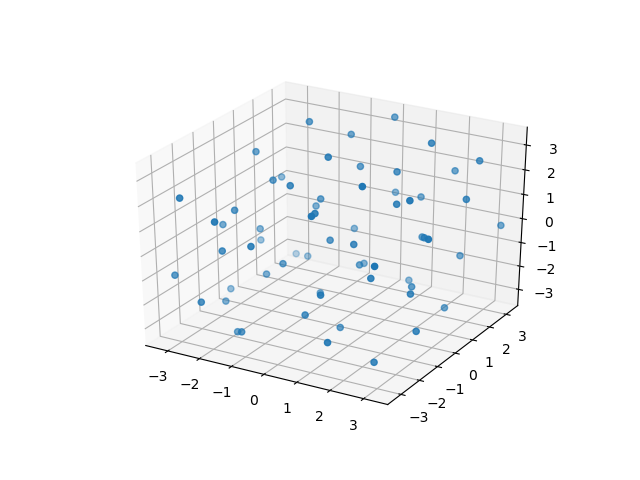
\includegraphics[width=0.8\textwidth]{fig/sim-1.png}
    \caption{-1:GLEQ}
\end{figure}
\begin{figure}[!htbp]
    \centering
    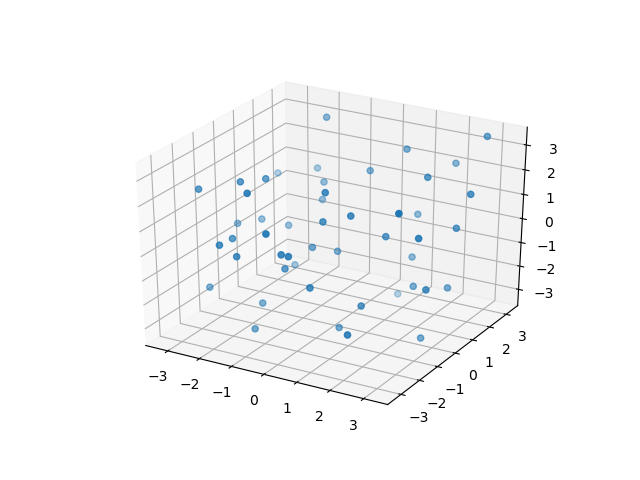
\includegraphics[width=0.8\textwidth]{fig/sim1.png}
    \caption{1:BERE修正力, 只用了3步就发散了}
\end{figure}
\begin{figure}[!htbp]
    \centering
    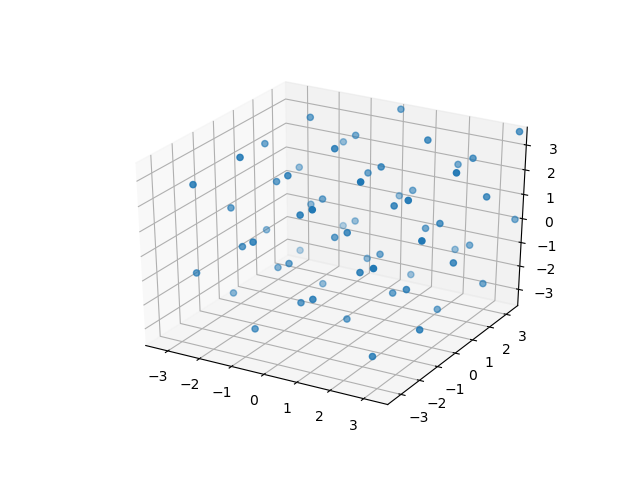
\includegraphics[width=0.8\textwidth]{fig/sim2.png}
    \caption{2:ZERO}
\end{figure}
\begin{figure}[!htbp]
    \centering
    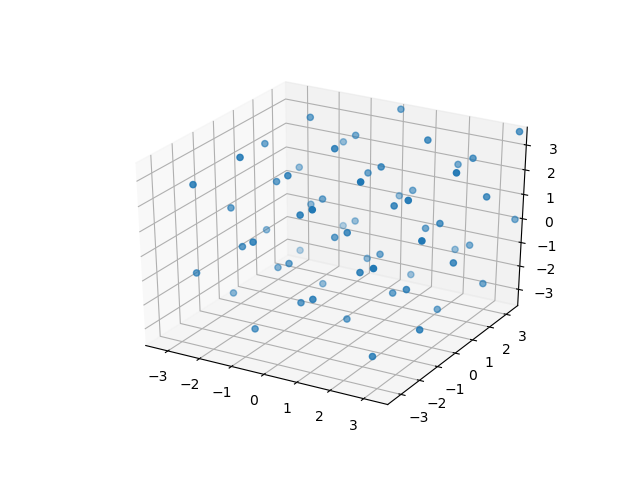
\includegraphics[width=0.8\textwidth]{fig/sim3.png}
    \caption{3:HOOV}
\end{figure}
\begin{figure}[!htbp]
    \centering
    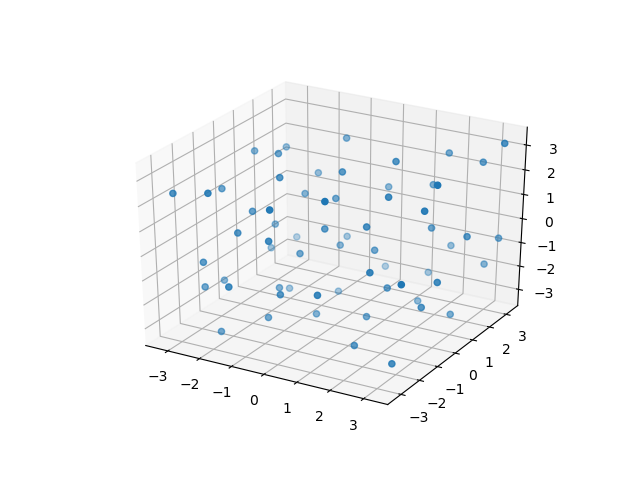
\includegraphics[width=0.8\textwidth]{fig/sim5.png}
    \caption{5:BERE修正速度}
\end{figure}
\begin{figure}[!htbp]
    \centering
    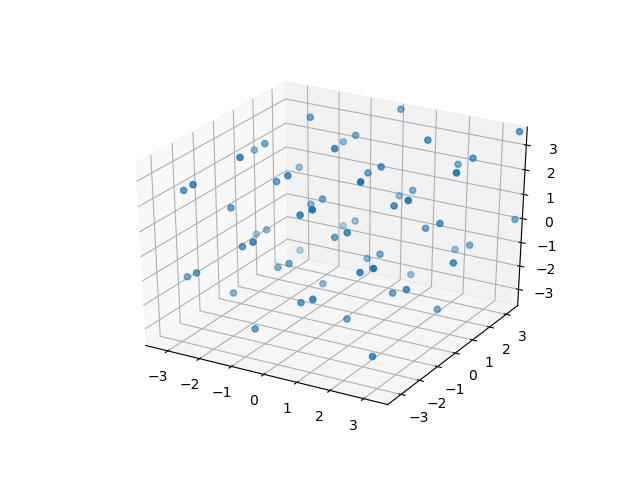
\includegraphics[width=0.8\textwidth]{fig/sim8.png}
    \caption{8:rescale}
\end{figure}

\section{总结}
我们研究了BrennerMD这一框架,对于FORTRAN 77有了更深的了解,同时也有一次对于分子动力学模拟有了更深刻的认识。
同时,我们也清楚地认识到,作为一名物理学研究者,使用程序语言清楚地表达自己地算法和思路是多么重要。

通过对于BrennerMD框架的阅读与对于FORTRAN 77语言的学习,我们本着对于历史人物的同情得出这样的结论:
FORTRAN 77的设计使得它完全无法胜任如此大规模程序的维护与扩展,同时,BrennerMD程序的组织与代码的混乱也给这一境况雪上加霜。
这个框架之所以用FORTRAN 77编写,完全是因为当时没有相同性能的其它高级编程语言,而不是因为FORTRAN 77自身的设计合理。
虽然在现代科学研究中,我们不再如此需要关注底层的框架是如何编写的,但是BrennerMD的bug过多,又不够健壮(robust),显然是不能胜任“基础框架”这一任务的。
这个框架除了用于教学,已经没有特别的科研价值了。

\section{分工}
\paragraph{王宇逸}概述、初始化、应用
\paragraph{谷海桥}计算、预测修正、恒温算法
\paragraph{李禹苏}能量最小化

\section{致谢}
感谢助教的帮助与同学们在群里的讨论。

感谢Intel。尽管我们并没有用到他们的编译器,但是不同编译器的结果不同,证明了FORTRAN 77写程序是多么不易。

\renewcommand{\refname}{参考文献}
\bibliography{report.bib}
\nocite{*}
\end{document}
